\documentclass[ignorenonframetext,aspectratio=169,]{paradise-slide}
\setbeamertemplate{caption}[numbered]
\setbeamertemplate{caption label separator}{:}
\setbeamercolor{caption name}{fg=normal text.fg}
\usepackage{amssymb,amsmath}
\usepackage{ifxetex,ifluatex}
\usepackage{fixltx2e} % provides \textsubscript

% use upquote if available, for straight quotes in verbatim environments
\IfFileExists{upquote.sty}{\usepackage{upquote}}{}
% use microtype if available
\IfFileExists{microtype.sty}{\usepackage{microtype}}{}
\usepackage{graphicx}
\makeatletter
\def\maxwidth{\ifdim\Gin@nat@width>\linewidth\linewidth\else\Gin@nat@width\fi}
\def\maxheight{\ifdim\Gin@nat@height>\textheight0.8\textheight\else\Gin@nat@height\fi}
\makeatother
% Scale images if necessary, so that they will not overflow the page
% margins by default, and it is still possible to overwrite the defaults
% using explicit options in \includegraphics[width, height, ...]{}
\setkeys{Gin}{width=\maxwidth,height=\maxheight,keepaspectratio}

% Comment these out if you don't want a slide with just the
% part/section/subsection/subsubsection title:
\AtBeginPart{
  \let\insertpartnumber\relax
  \let\partname\relax
  \frame{\partpage}
}
\AtBeginSection{
  \let\insertsectionnumber\relax
  \let\sectionname\relax
  \frame{\sectionpage}
}
\AtBeginSubsection{
  \let\insertsubsectionnumber\relax
  \let\subsectionname\relax
  \frame{\subsectionpage}
}

\setlength{\parindent}{0pt}
\setlength{\emergencystretch}{3em}  % prevent overfull lines
\providecommand{\tightlist}{%
  \setlength{\itemsep}{0pt}\setlength{\parskip}{0pt}}
\setcounter{secnumdepth}{0}
\ifxetex
  \usepackage{polyglossia}
  \setmainlanguage{}
  \setotherlanguages{}
\else
  \usepackage[shorthands=off,english]{babel}
\fi
\usepackage{pgf, pgffor}
\usepackage{listings}
\usepackage{mathtools}
\usepackage{booktabs}
\usepackage{dirtytalk}
\newcommand{\columnsbegin}{\begin{columns}}
\newcommand{\columnsend}{\end{columns}}

\title{Comparison of A* and RRT-Connect Motion Planning Techniques for
Self-Reconfiguration Planning}
\author{David Brandt \and \linebreak \and \linebreak \and presented by Jan Mrázek}
\date{26th October 2020}

\begin{document}
\frame[plain]{\titlepage}

\begin{frame}[fragile]{The Problem of Reconfiguration}
\protect\hypertarget{the-problem-of-reconfiguration}{}

\begin{itemize}
\tightlist
\item
  given an initial and target configuration

  \begin{itemize}
  \tightlist
  \item
    structure
  \item
    position in space
  \end{itemize}
\item
  find a sequence of atomic actions that lead from the initial to the
  target configuration

  \begin{itemize}
  \tightlist
  \item
    collision-free
  \item
    feasible (e.g., consider limited strength of joints)
  \item
    optimal vs.~feasible solution
  \end{itemize}
\end{itemize}

\pause

\textbf{This paper:}

\begin{itemize}
\tightlist
\item
  tackles reconfiguration for ATRONs
\item
  uses state-space search

  \begin{itemize}
  \tightlist
  \item
    A*
  \item
    RRT-Connect
  \end{itemize}
\item
  provides comparison
\end{itemize}

\end{frame}

\begin{frame}[fragile]{ATRONs}
\protect\hypertarget{atrons}{}

\begin{figure}
\centering
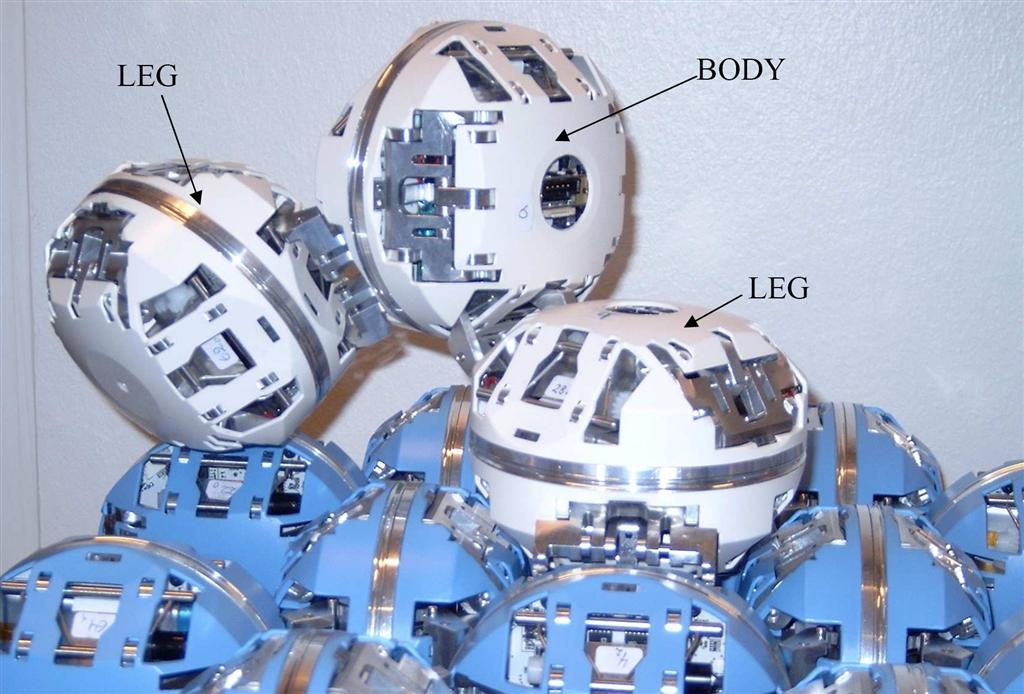
\includegraphics{atron.jpg}
\caption{ATRON}
\end{figure}

\end{frame}

\begin{frame}[fragile]{Sidenote}
\protect\hypertarget{sidenote}{}

\begin{itemize}
\tightlist
\item
  state-space of reconfiguration have high number of dimensions
\item
  all algorithms we will present work on unlimited number of dimensions
\item
  we will illustrate them in 2D for simplicity
\end{itemize}

\end{frame}

\begin{frame}[fragile]{Preliminary: Probabilistic Road Map Planners}
\protect\hypertarget{preliminary-probabilistic-road-map-planners}{}

\begin{columns}

\column{.45\textwidth}

\begin{itemize}
\tightlist
\item
  build a discrete graph over the state space by random sampling
\item
  use, e.g., Dijkstra to find shortest paths in the discrete graph
\end{itemize}

\textbf{Building the graph:}

\begin{itemize}
\tightlist
\item
  take random configuration
\item
  if invalid, discard
\item
  find path to an already sampled points

  \begin{itemize}
  \tightlist
  \item
    when not found - discard
  \item
    add new vertex and edge to the graph
  \item
    use heuristics
  \end{itemize}
\item
  repeat until dense enough graph is built
\end{itemize}

\column{.4\textwidth}

\begin{figure}
\centering
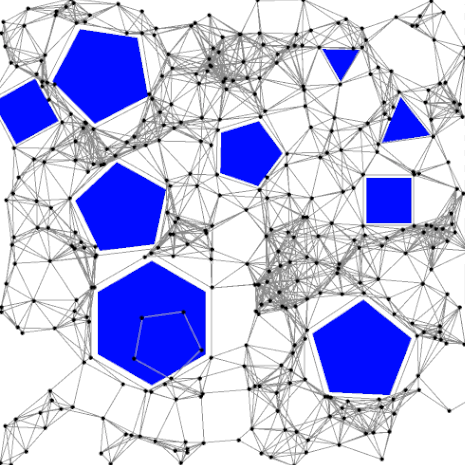
\includegraphics{PRM-23.png}
\caption{Discrete navigation graph}
\end{figure}

\end{columns}

\end{frame}

\begin{frame}[fragile]{Preliminary: Navigation Graph}
\protect\hypertarget{preliminary-navigation-graph}{}

\begin{figure}
\centering
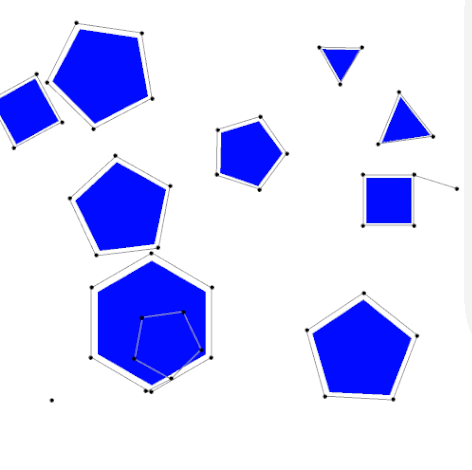
\includegraphics{PRM-0.png}
\caption{Step 1 (Source Wikipedia)}
\end{figure}

\end{frame}

\begin{frame}[fragile]{Preliminary: Navigation Graph}
\protect\hypertarget{preliminary-navigation-graph-1}{}

\begin{figure}
\centering
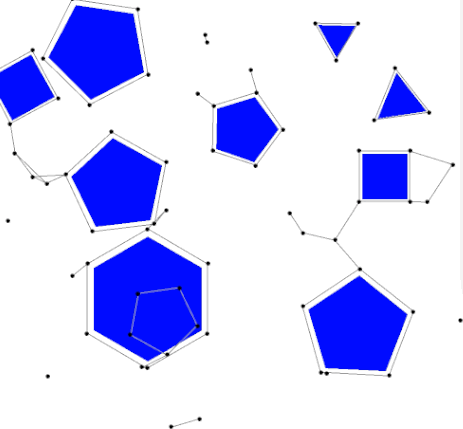
\includegraphics{PRM-1.png}
\caption{Step 2 (Source Wikipedia)}
\end{figure}

\addtocounter{framenumber}{-1}

\end{frame}

\begin{frame}[fragile]{Preliminary: Navigation Graph}
\protect\hypertarget{preliminary-navigation-graph-2}{}

\begin{figure}
\centering
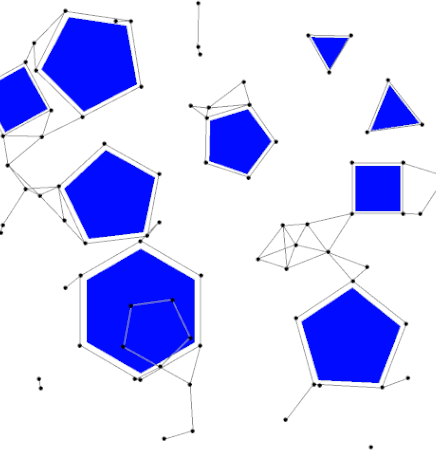
\includegraphics{PRM-2.png}
\caption{Step 3 (Source Wikipedia)}
\end{figure}

\addtocounter{framenumber}{-1}

\end{frame}

\begin{frame}[fragile]{Preliminary: Navigation Graph}
\protect\hypertarget{preliminary-navigation-graph-3}{}

\begin{figure}
\centering
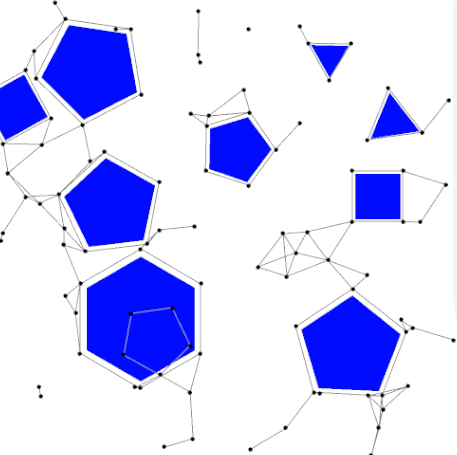
\includegraphics{PRM-3.png}
\caption{Step 4 (Source Wikipedia)}
\end{figure}

\addtocounter{framenumber}{-1}

\end{frame}

\begin{frame}[fragile]{Preliminary: Navigation Graph}
\protect\hypertarget{preliminary-navigation-graph-4}{}

\begin{figure}
\centering
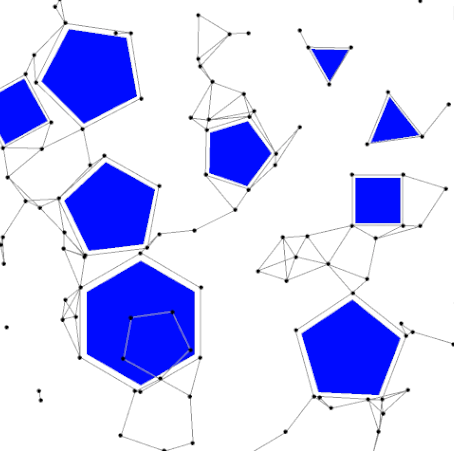
\includegraphics{PRM-4.png}
\caption{Step 5 (Source Wikipedia)}
\end{figure}

\addtocounter{framenumber}{-1}

\end{frame}

\begin{frame}[fragile]{Preliminary: Navigation Graph}
\protect\hypertarget{preliminary-navigation-graph-5}{}

\begin{figure}
\centering
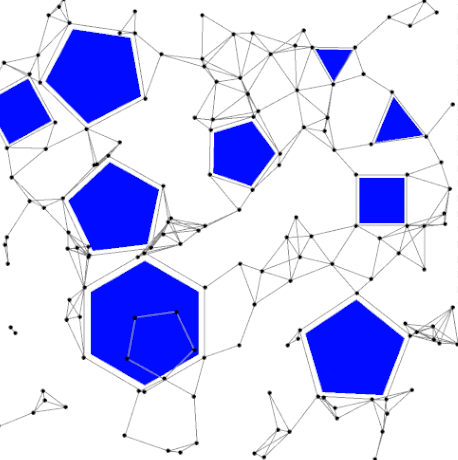
\includegraphics{PRM-7.png}
\caption{Step 6 (Source Wikipedia)}
\end{figure}

\addtocounter{framenumber}{-1}

\end{frame}

\begin{frame}[fragile]{Preliminary: Navigation Graph}
\protect\hypertarget{preliminary-navigation-graph-6}{}

\begin{figure}
\centering
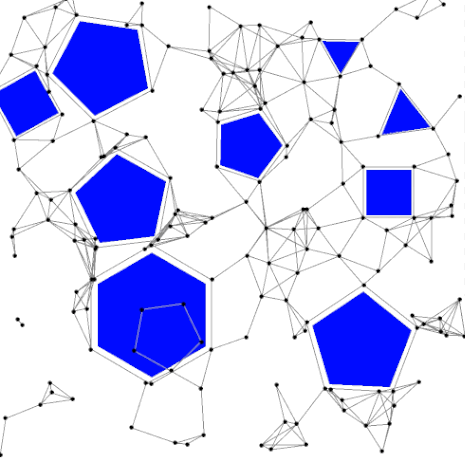
\includegraphics{PRM-8.png}
\caption{Step 7 (Source Wikipedia)}
\end{figure}

\addtocounter{framenumber}{-1}

\end{frame}

\begin{frame}[fragile]{Preliminary: RRT}
\protect\hypertarget{preliminary-rrt}{}

\begin{columns}

\column{.3\textwidth}

\begin{itemize}
\tightlist
\item
  find only path to the nearest point
\item
  \(\rightarrow\) tree
\end{itemize}

\column{.7\textwidth}

\begin{figure}
\centering
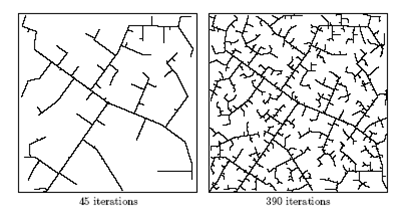
\includegraphics{RRT_graph1.png}
\caption{RRT (Source Wikipedia)}
\end{figure}

\end{columns}

\end{frame}

\begin{frame}[fragile]{RRT-Connect}
\protect\hypertarget{rrt-connect}{}

\begin{columns}

\column{.4\textwidth}

\textbf{It is hard to a find path between two configurations}

\begin{itemize}
\tightlist
\item
  make only a step towards random configuration
\item
  build two trees and try to connect them
\end{itemize}

\column{.6\textwidth}

\begin{figure}
\centering
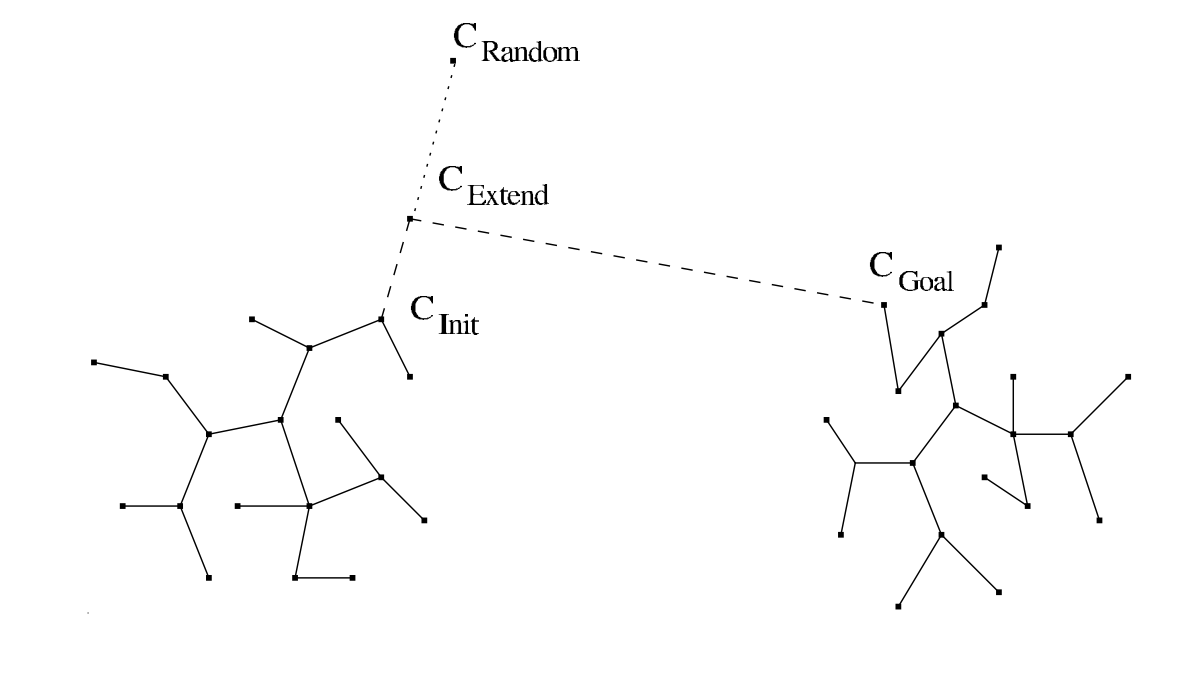
\includegraphics{rrtconect.png}
\caption{RRT - Connect}
\end{figure}

\end{columns}

\pause

\textbf{What is \say{a step towards a configuration?}}

\end{frame}

\begin{frame}[fragile]{Configuration Similarity Metric}
\protect\hypertarget{configuration-similarity-metric}{}

\begin{itemize}
\tightlist
\item
  optimal solution: minimal number of atomic steps to change one
  configuration to another

  \begin{itemize}
  \tightlist
  \item
    the problem is NP-complete (proven in 2016)
  \end{itemize}
\end{itemize}

\pause

\textbf{Approximation:}

\begin{equation*}
    \text{dist}(a_1, a_2) = \text{max}(|a_{1_x}, a_{2_x}|, |a_{1_y}, a_{2_y}|, |a_{1_z}, a_{2_z}|)
    + \frac{\text{diffOri}(a_1, a_2)}{2} + \frac{\text{diffConn}(a_1, a_2)}{16}
\end{equation*} where: \begin{equation*}
    \text{diffOri}(a_1, a_2) =
    \begin{cases*}
      1 & if orientation of $a_1$ differs from $a_2$ \\
      0 & otherwise
    \end{cases*}
\end{equation*}

\begin{equation*}
    \text{diffConn}(a_1, a_2) = \text{number of connectors in different state}
\end{equation*}

Find pairing of modules from one configuration the other minimizing sum
of distances

\end{frame}

\begin{frame}[fragile]{Hungarian Algorithm}
\protect\hypertarget{hungarian-algorithm}{}

\begin{itemize}
\tightlist
\item
  solve assignment between workers and tasks
\item
  input is matrix \(n\times n\):
\end{itemize}

\begin{table}[]
\begin{tabular}{@{}rccc@{}}
\toprule
               & \textbf{Clean bathroom} & \textbf{Sweep floors} & \textbf{Wash windows} \\ \midrule
\textbf{Paul}  & 2\$                     & 3\$                   & 3\$                   \\
\textbf{Dave}  & 3\$                     & 2\$                   & 3\$                   \\
\textbf{Chris} & 3\$                     & 3\$                   & 2\$                   \\ \bottomrule
\end{tabular}
\end{table}

\begin{itemize}
\tightlist
\item
  minimum cost: \$6

  \begin{itemize}
  \tightlist
  \item
    Paul clean the bathroom
  \item
    Dave sweep the floors
  \item
    Chris wash the windows
  \end{itemize}
\item
  runs in \(\mathcal{O}(n^3)\)
\end{itemize}

\end{frame}

\begin{frame}[fragile]{Configuration Similarity Metric: Putting it All Together}
\protect\hypertarget{configuration-similarity-metric-putting-it-all-together}{}

\begin{itemize}
\tightlist
\item
  prepare matrix \(n\times n\) representing possible pairings

  \begin{itemize}
  \tightlist
  \item
    values in the matrix are \(\text{dist}(a_x, a_y)\)
  \item
    can be computed in \(\mathcal{O}(n^2)\)
  \end{itemize}
\item
  find the minimal pairing using the Hungarian algorithm

  \begin{itemize}
  \tightlist
  \item
    can be computed in \(\mathcal{O}(n^3)\)
  \end{itemize}
\end{itemize}

\end{frame}

\begin{frame}[fragile]{RRT-Connect on ATRONs}
\protect\hypertarget{rrt-connect-on-atrons}{}

\begin{columns}

\column{.4\textwidth}

\begin{itemize}
\tightlist
\item
  finding optimal \(C_{Extend}\) is expensive
\item
  the authors use 3 atomic steps as an approximation
\end{itemize}

\column{.6\textwidth}

\begin{figure}
\centering
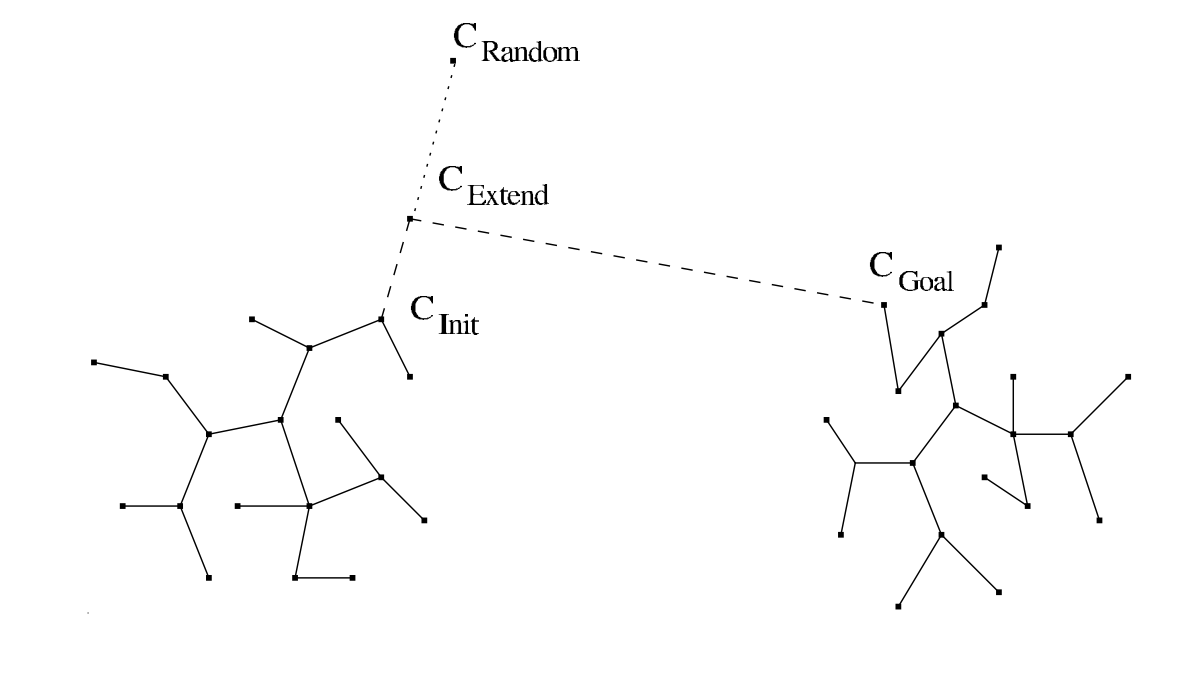
\includegraphics{rrtconect.png}
\caption{RRT - Connect}
\end{figure}

\end{columns}

\end{frame}

\begin{frame}[fragile]{Recap: A*}
\protect\hypertarget{recap-a}{}

\begin{itemize}
\tightlist
\item
  create a set \texttt{open} with the initial configuration
\item
  create an empty set \texttt{closed}
\item
  repeat until \texttt{open} is not empty and path have not been found:

  \begin{itemize}
  \tightlist
  \item
    get a configuration from \texttt{open} that is closest to the target
    configuration
  \item
    if the distance is zero, path have been found
  \item
    generate all successors and put them \texttt{open} if they are not
    in \texttt{closed}
  \item
    put configuration into \texttt{closed}
  \end{itemize}
\end{itemize}

Successors are generated as a sequence of 3 atomic steps to overcome
small local minima.

\end{frame}

\begin{frame}[fragile]{Comparison}
\protect\hypertarget{comparison}{}

\begin{figure}
\centering
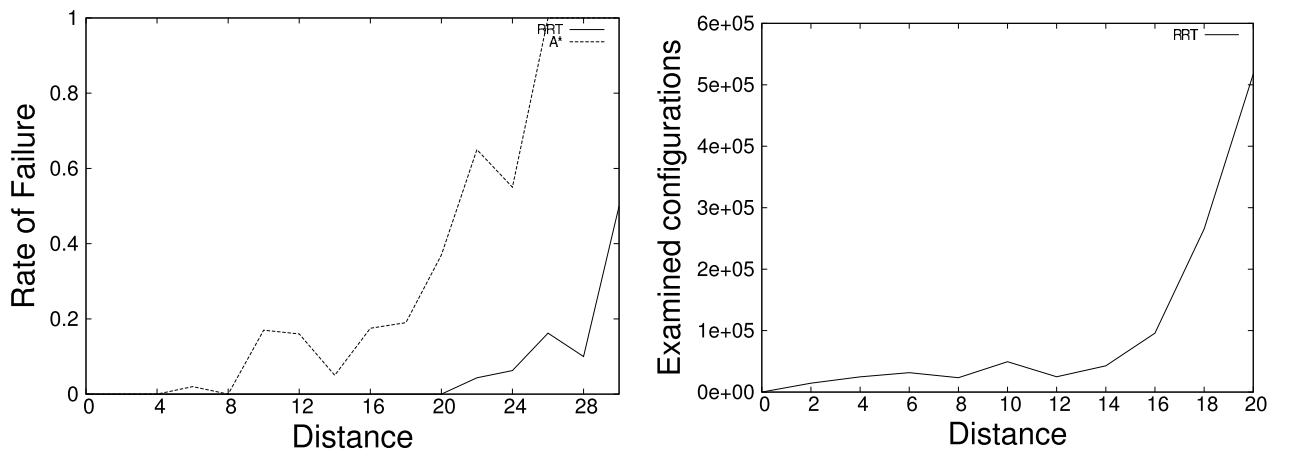
\includegraphics{results.png}
\caption{Results}
\end{figure}

\begin{itemize}
\tightlist
\item
  limit \(10^7\) states examined (\textasciitilde30 minutes of compute
  time)
\item
  note the clear exponential increase in examined states
\end{itemize}

\end{frame}

\begin{frame}[fragile]{Conclusion}
\protect\hypertarget{conclusion}{}

\begin{itemize}
\tightlist
\item
  RRT-Connect can be perceived as \say{randomized A*}

  \begin{itemize}
  \tightlist
  \item
    it helps to move to another location before examining the whole
    local minima
  \end{itemize}
\item
  A* finds optimal solution, RRT-Connect finds long paths

  \begin{itemize}
  \tightlist
  \item
    RRT paths can be post-processed
  \end{itemize}
\end{itemize}

\pause

\textbf{What might be interesting for RoFI:}

\begin{itemize}
\tightlist
\item
  ignore module ids by performing matching
\item
  came up with similar similarity metrics

  \begin{itemize}
  \tightlist
  \item
    experimentally fine-tune parameters
  \end{itemize}
\item
  implement RRT-Connect and benchmark it
\end{itemize}

\end{frame}

\end{document}
